\begin{frame}[label=interferometry]
    \frametitle{How Do We Locate Meteors?}
    \begin{columns}
        \begin{column}{0.7\textwidth}
            \begin{center}
                \begin{alertblock}{Interferometry}
                    Using an \textbf{array of antennas}, differences  in signals’ \textbf{phase} are used to determine the \textbf{direction to the meteor} 
                \end{alertblock}
            \end{center}

            This requires an array of 5+ antennas
            \begin{itemize}
                \item Array geometry is \textit{precisely} known
                \item Each antenna sends out a unique signal
                \item The \alert{phase} of each signal is synchronized 
            \end{itemize}
        \end{column}
        \begin{column}{0.3\textwidth}
            \begin{tikzpicture}
                \node[anchor=center, inner sep=0] (img) at (0,0) {
                    {{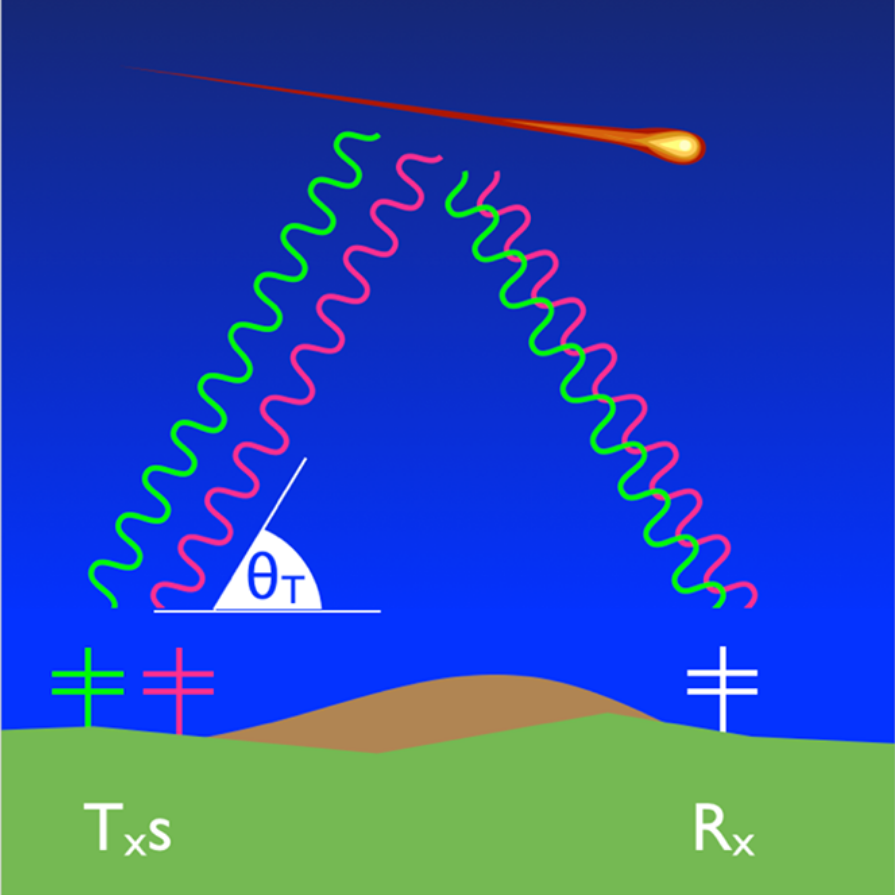
\includegraphics[width=\linewidth]{img/aoa_aod.png}}}
                };
                \node[anchor=north east, inner sep=2pt] at (img.north east) { 
                    {{{\fontsize{3}{3.4}\selectfont\raggedleft \textcolor{white}{\textit{Credit:} \citeauthor{chau_NovelSpecularMeteor_2019}, \citeyear{chau_NovelSpecularMeteor_2019}\cite{chau_NovelSpecularMeteor_2019}}}}}
                };
                \node[anchor=north, inner sep=0] (img2) at ([yshift=-0.1cm]img.south) {
                    {{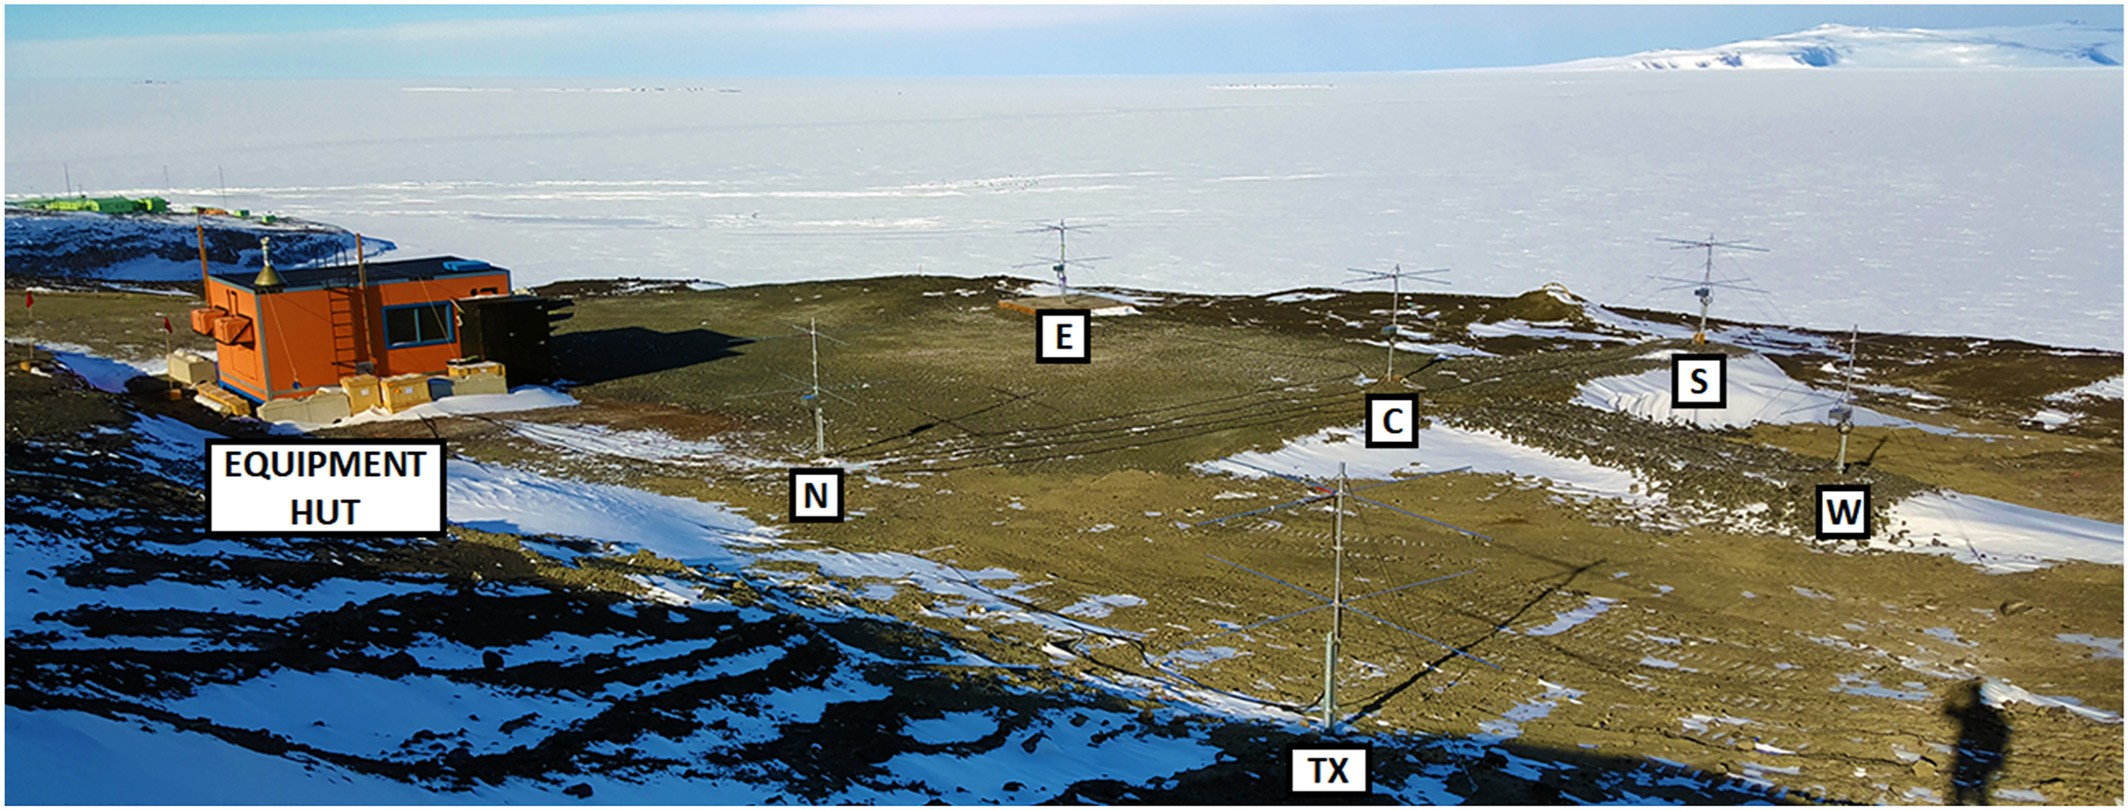
\includegraphics[width=\linewidth]{img/mcmurdo.jpg}}}
                };
                \node[anchor=north east, inner sep=2pt] at (img2.north east) { 
                    {{{\fontsize{3}{3.4}\selectfont\raggedleft \textcolor{black}{\textit{Credit:} \citeauthor{marino_FirstObservationsNew_2022}, \citeyear{marino_FirstObservationsNew_2022} \cite{marino_FirstObservationsNew_2022}}}}}
                };
            \end{tikzpicture}            
        \end{column}
    \end{columns}
\end{frame}




